\section{Bus CAN}
\subsection{Definición}
\begin{frame}
	\frametitle{Bus CAN}
    \begin{columns}[T]
    	\begin{column}{.5\textwidth}
    		% \centering
    		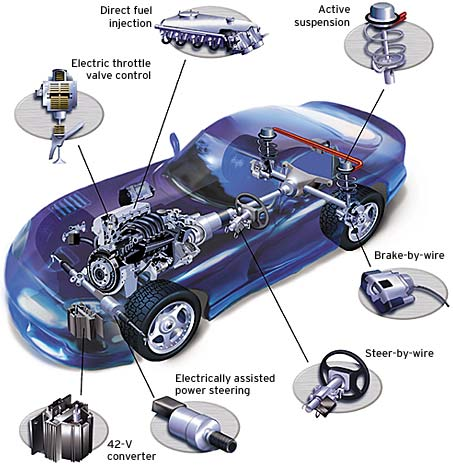
\includegraphics[scale=0.4]{images/ProtocoloCANAuto.png}
    	\end{column}
    	\begin{column}{.5\textwidth}
			\begin{itemize}
				\item Comenzó su desarrollo en 1983
				\item Estandarizado por la ISO (ISO 11898)
				\item Nació para ser usada en la industria automotriz
				\item Conectividad vía bus serial, a través de dos cables. 
				\item \textbf{Bajo costo}
			\end{itemize}
    	\end{column}
	\end{columns}
\end{frame}

\begin{frame}
	\frametitle{¿Por qué CAN Bus?}
	\vfill
	\begin{columns}[T]
		\begin{column}{.45\textwidth}
			\centering
			\vspace*{1cm}
			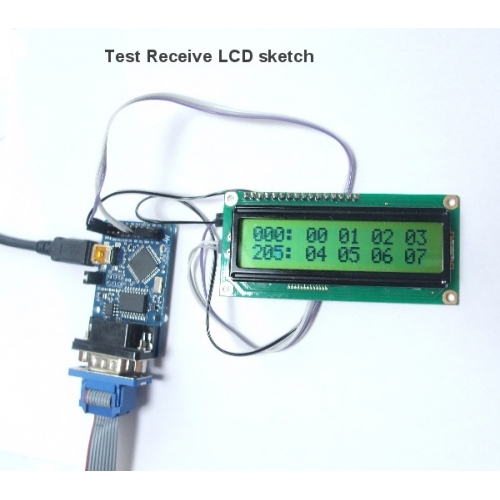
\includegraphics[scale=0.3]{images/bus_can.png}
		\end{column}
	    \begin{column}{.10\textwidth}
			\vspace*{3cm}
	    	\centering
	    	VS.
	    \end{column}
		\begin{column}{.45\textwidth}
			\centering
			\vspace*{2cm}
            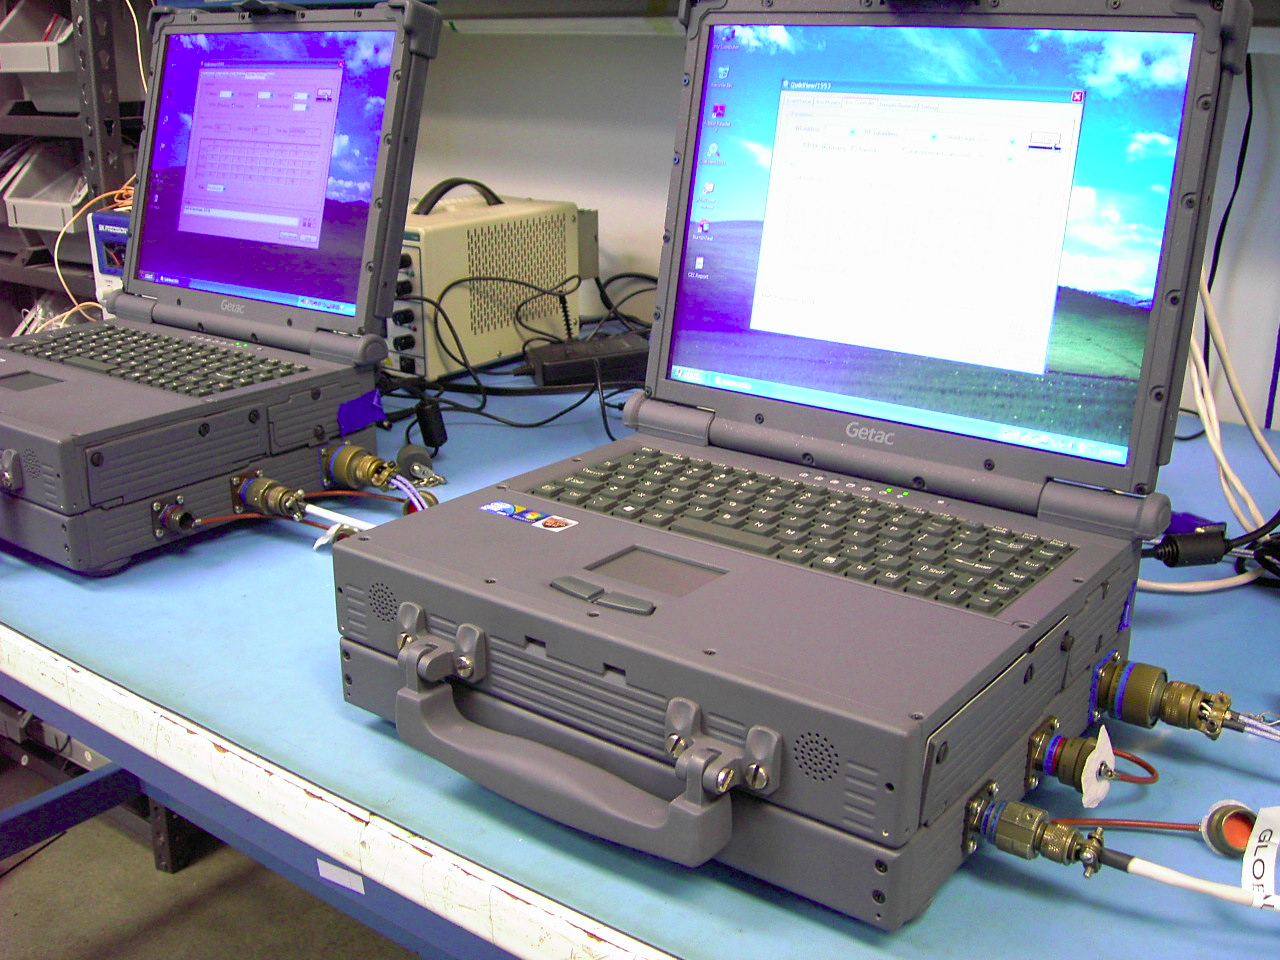
\includegraphics[scale=0.1]{images/1553.png}
		\end{column}
	\end{columns}
\end{frame}

\subsection{Protocolo CAN}
\begin{frame}
	\frametitle{Protocolo CAN}
	\begin{columns}[T]
		\begin{column}{.5\textwidth}
			\centering
			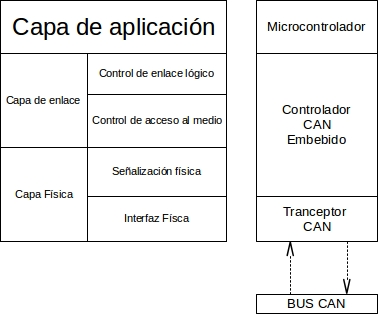
\includegraphics[scale=0.4]{images/ISO11898_Arquitectura_Standar.jpg}
		\end{column}
	    \begin{column}{.5\textwidth}
			\begin{table}[]
				\centering
				\begin{tabular}{c}
					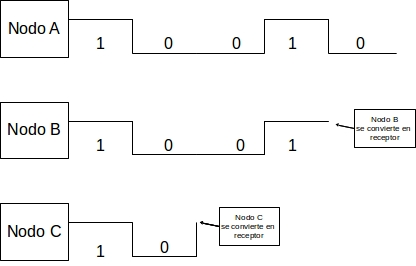
\includegraphics[scale=0.3]{images/CAN_BUS_Traffic.jpg} \\
					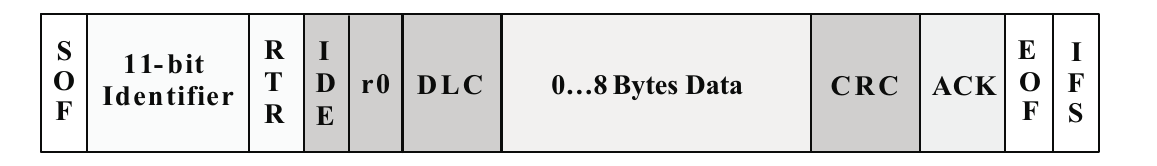
\includegraphics[scale=0.1]{images/StandarCAN.png} \\
					CAN Estándar \\ \hline
					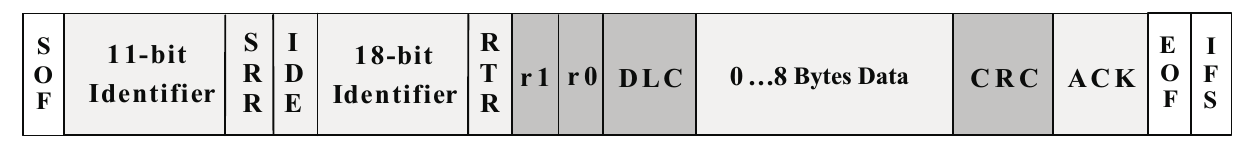
\includegraphics[scale=0.1]{images/ExtendedCAN.png} \\
					CAN Extendido \\
					\hline				
				\end{tabular}
			\end{table}
	    \end{column}
	\end{columns}
\end{frame}